\documentclass{article}
\usepackage{graphicx}
\begin{document}
	
	\section*{Lsg Vorschlag RUT Ü05 Maximilian Maag}
	\subsection*{Aufgagbe 5.1}
	\subsection*{a)}
	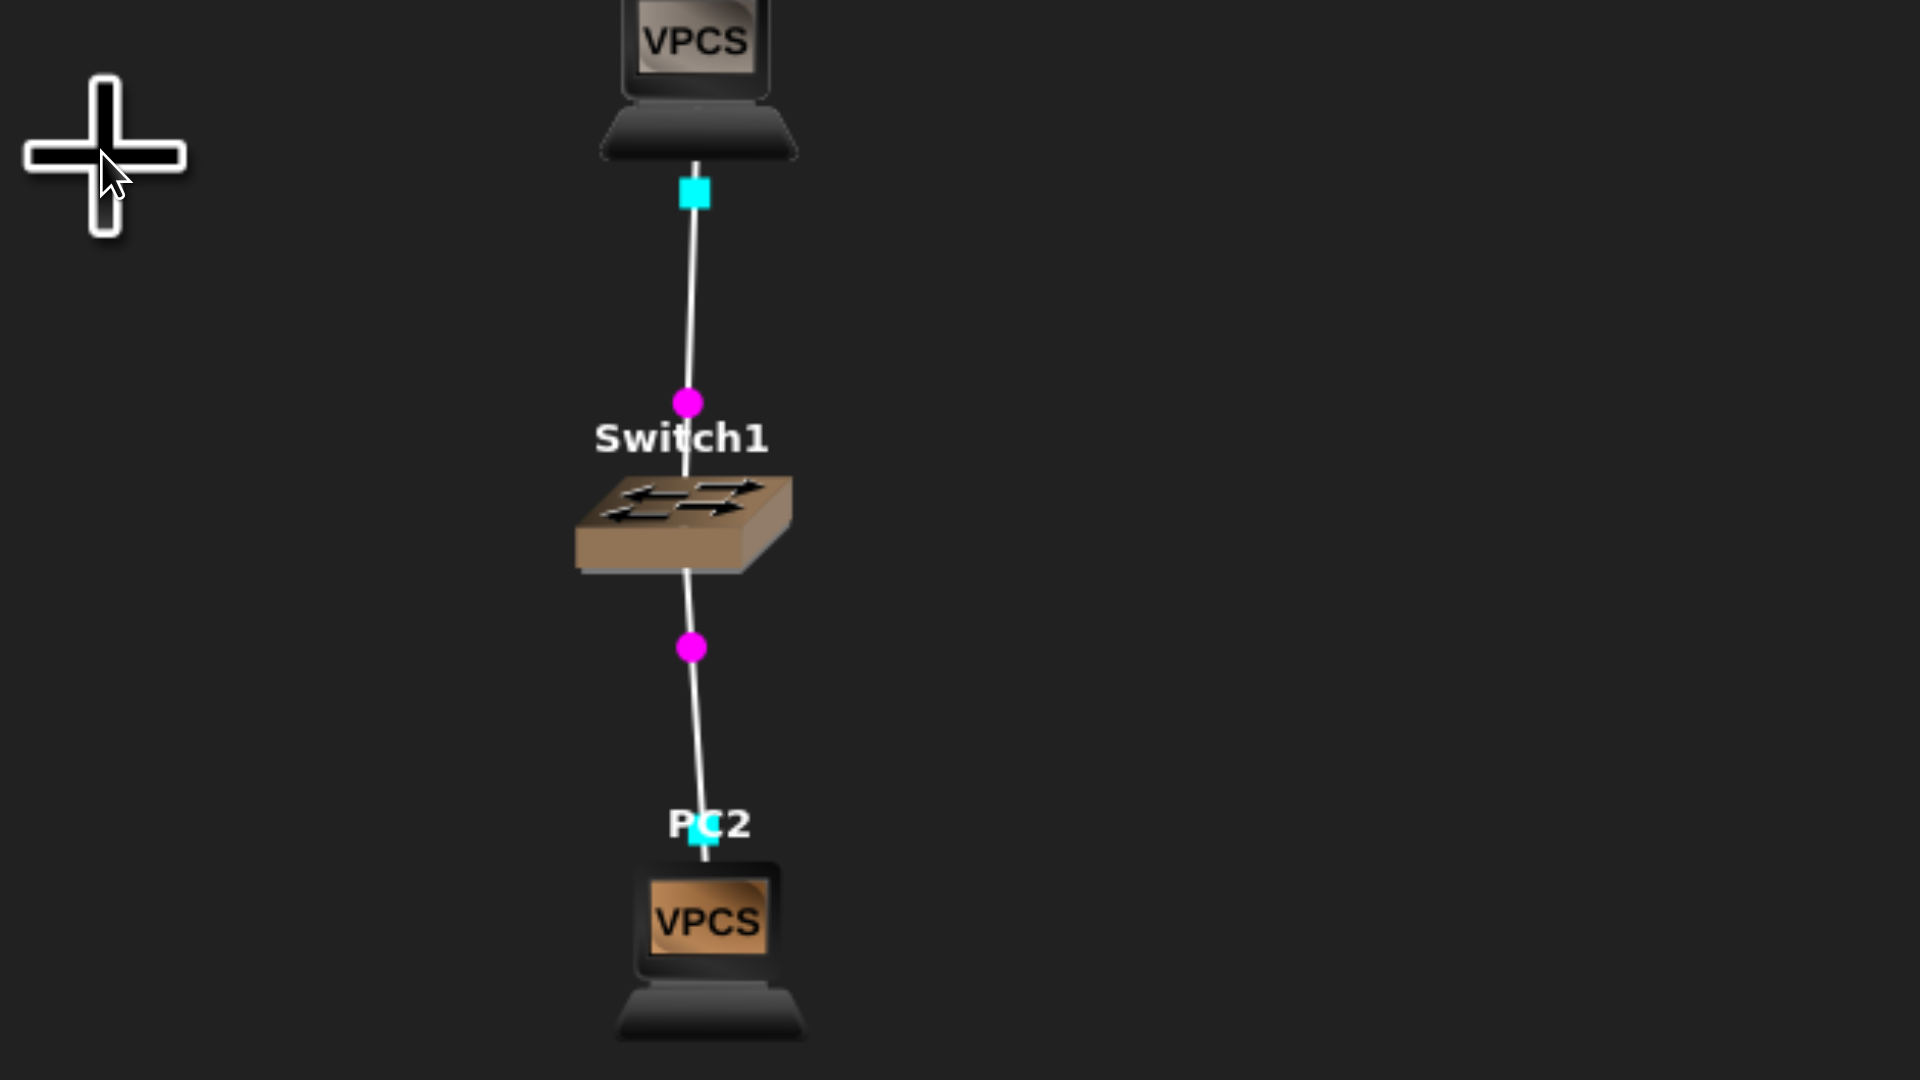
\includegraphics[width=\linewidth]{0501a}
	\subsection*{b)}
	IP Adresse auf PC1 \\
	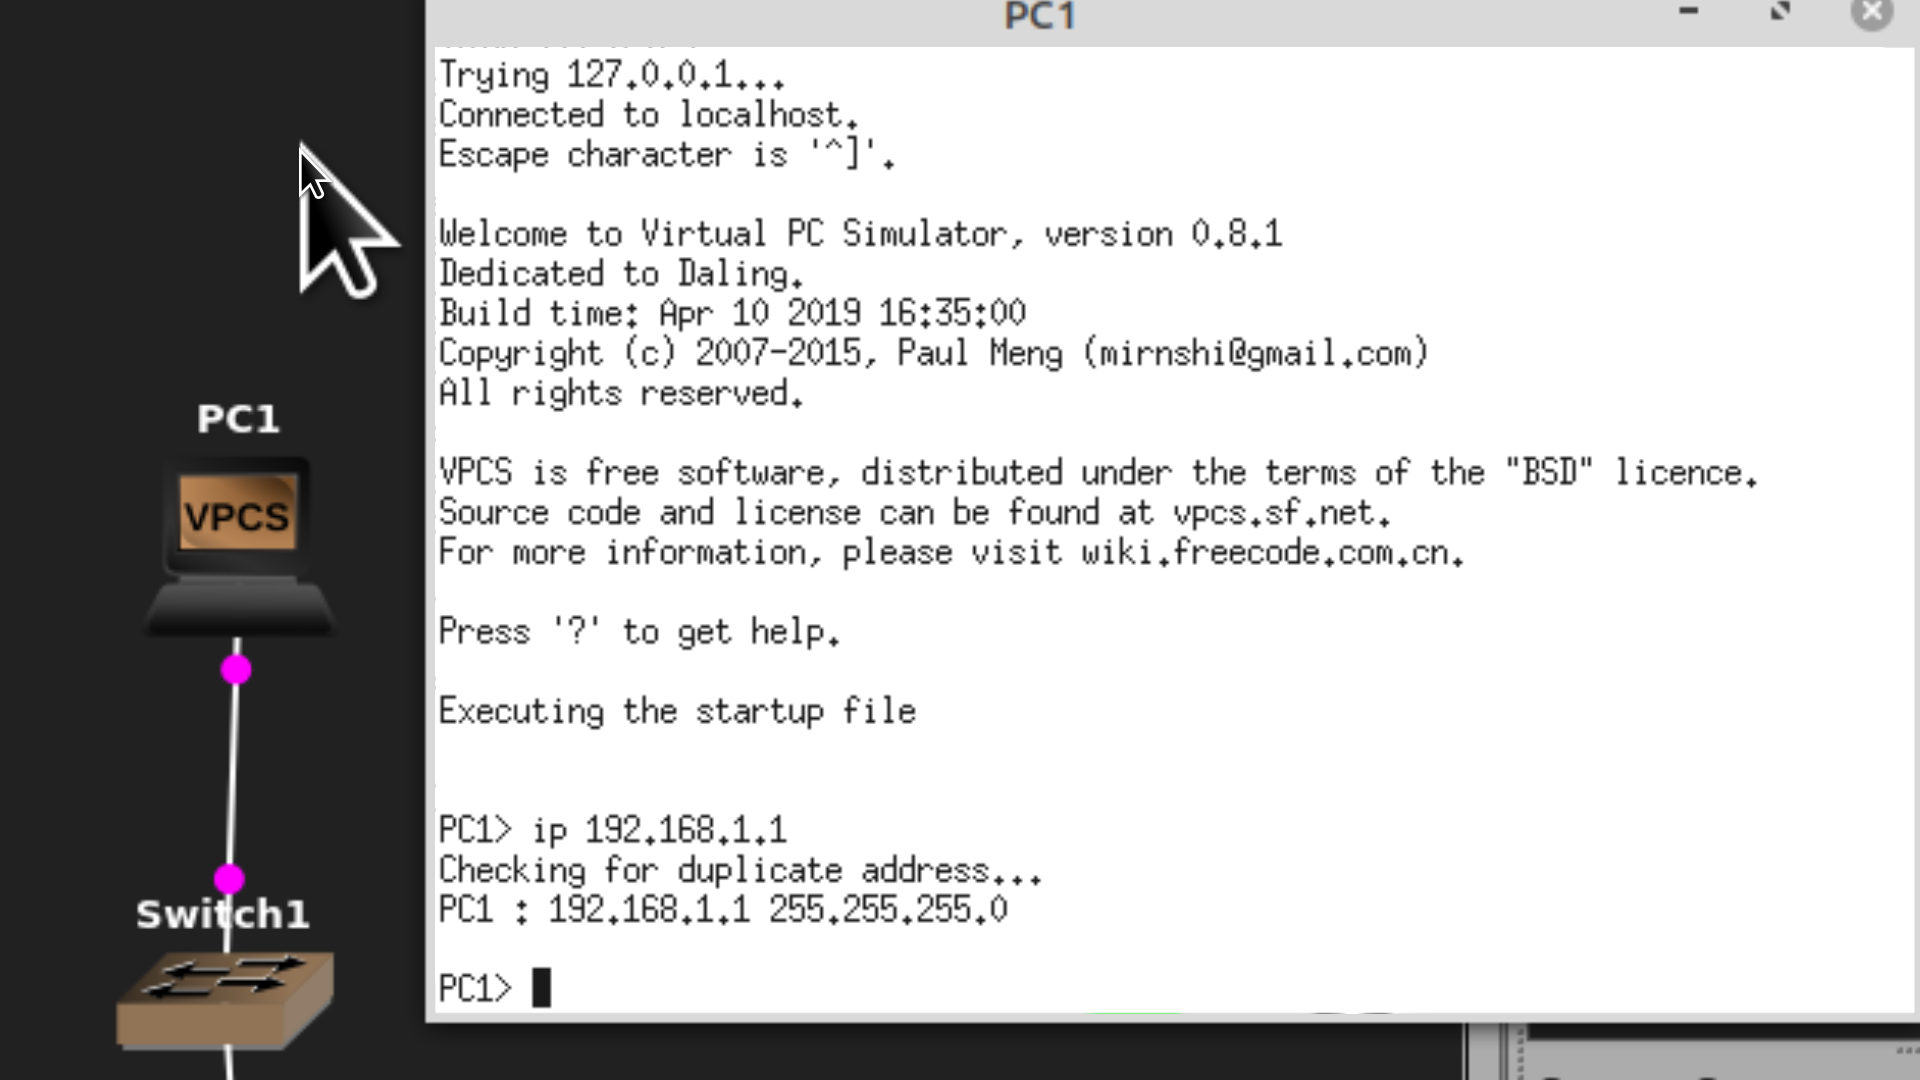
\includegraphics[width=\linewidth]{0501b01} \\ \\
	IP Adresse auf PC2 \\
	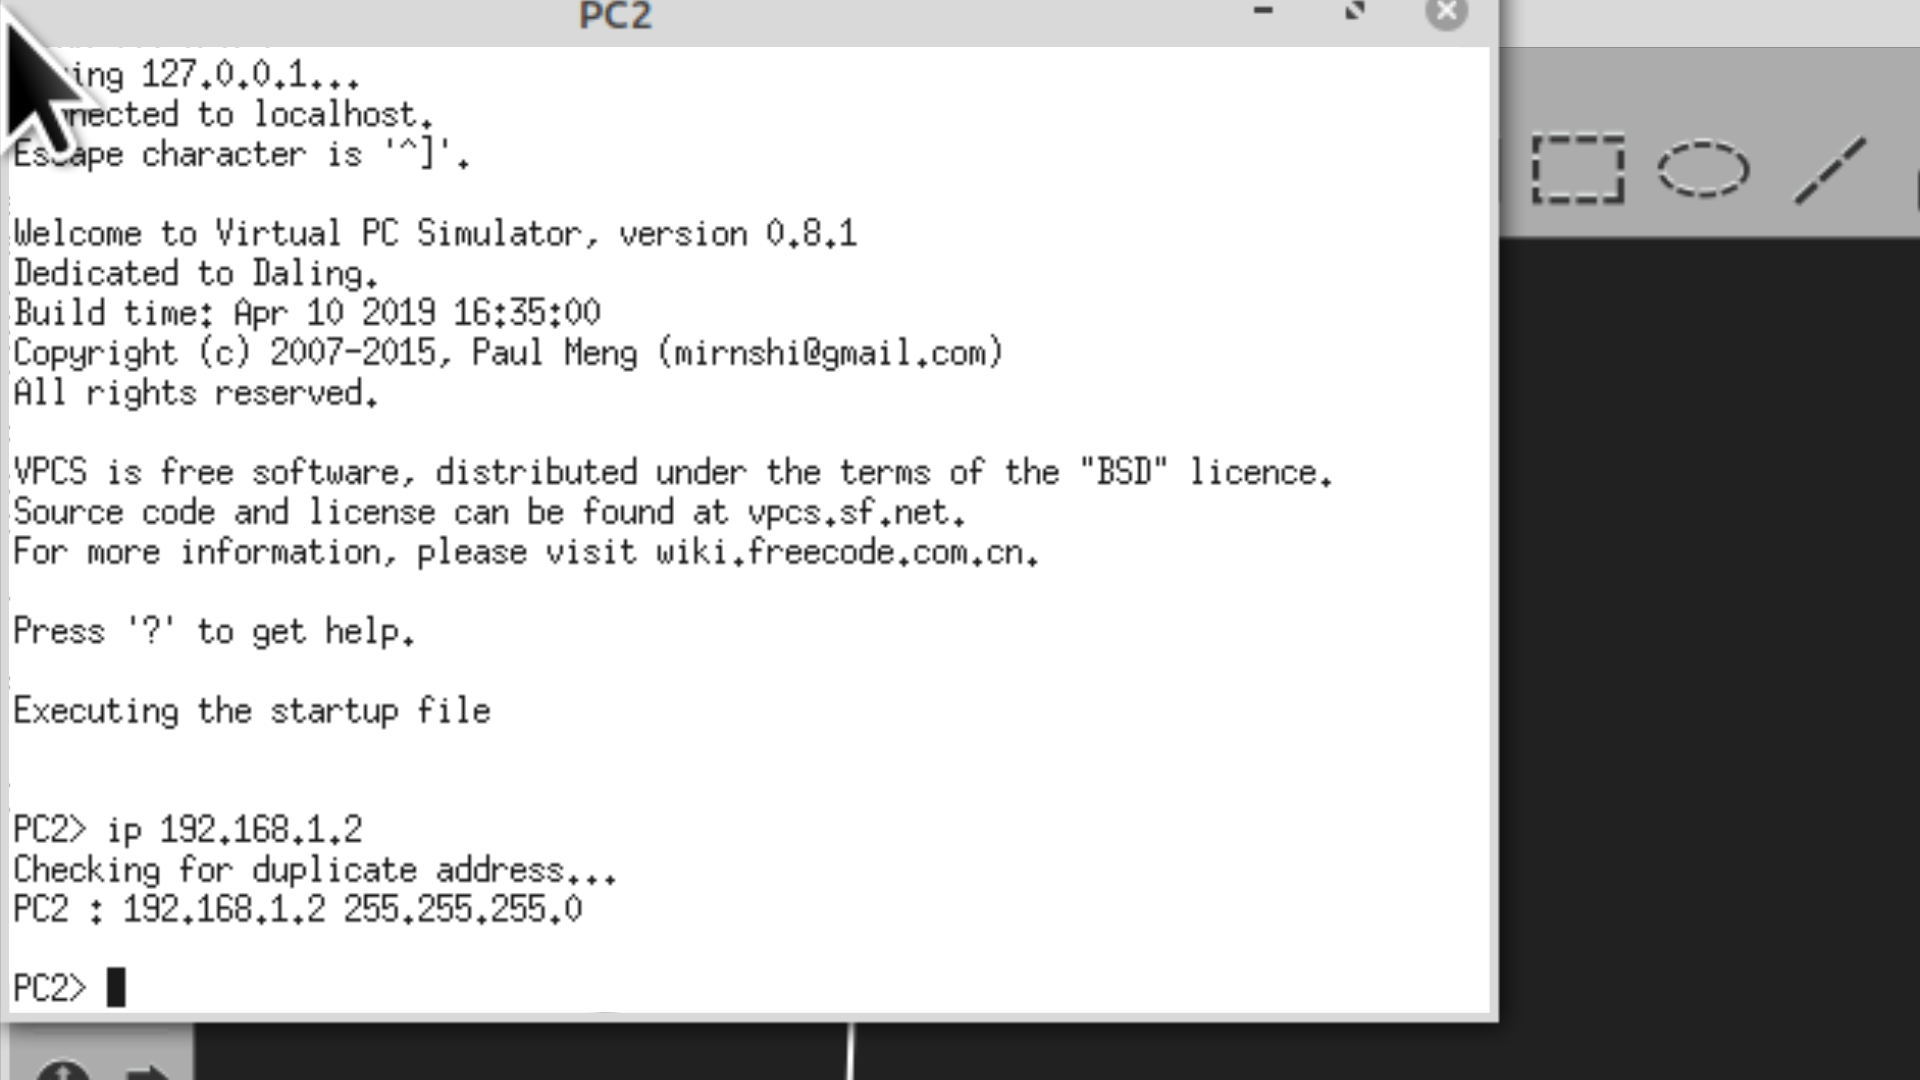
\includegraphics[width=\linewidth]{0501b02} \\ \\
	\subsection*{c)}
	Ping von PC1 nach PC2 aufgezeichnet mit WireShark \\
	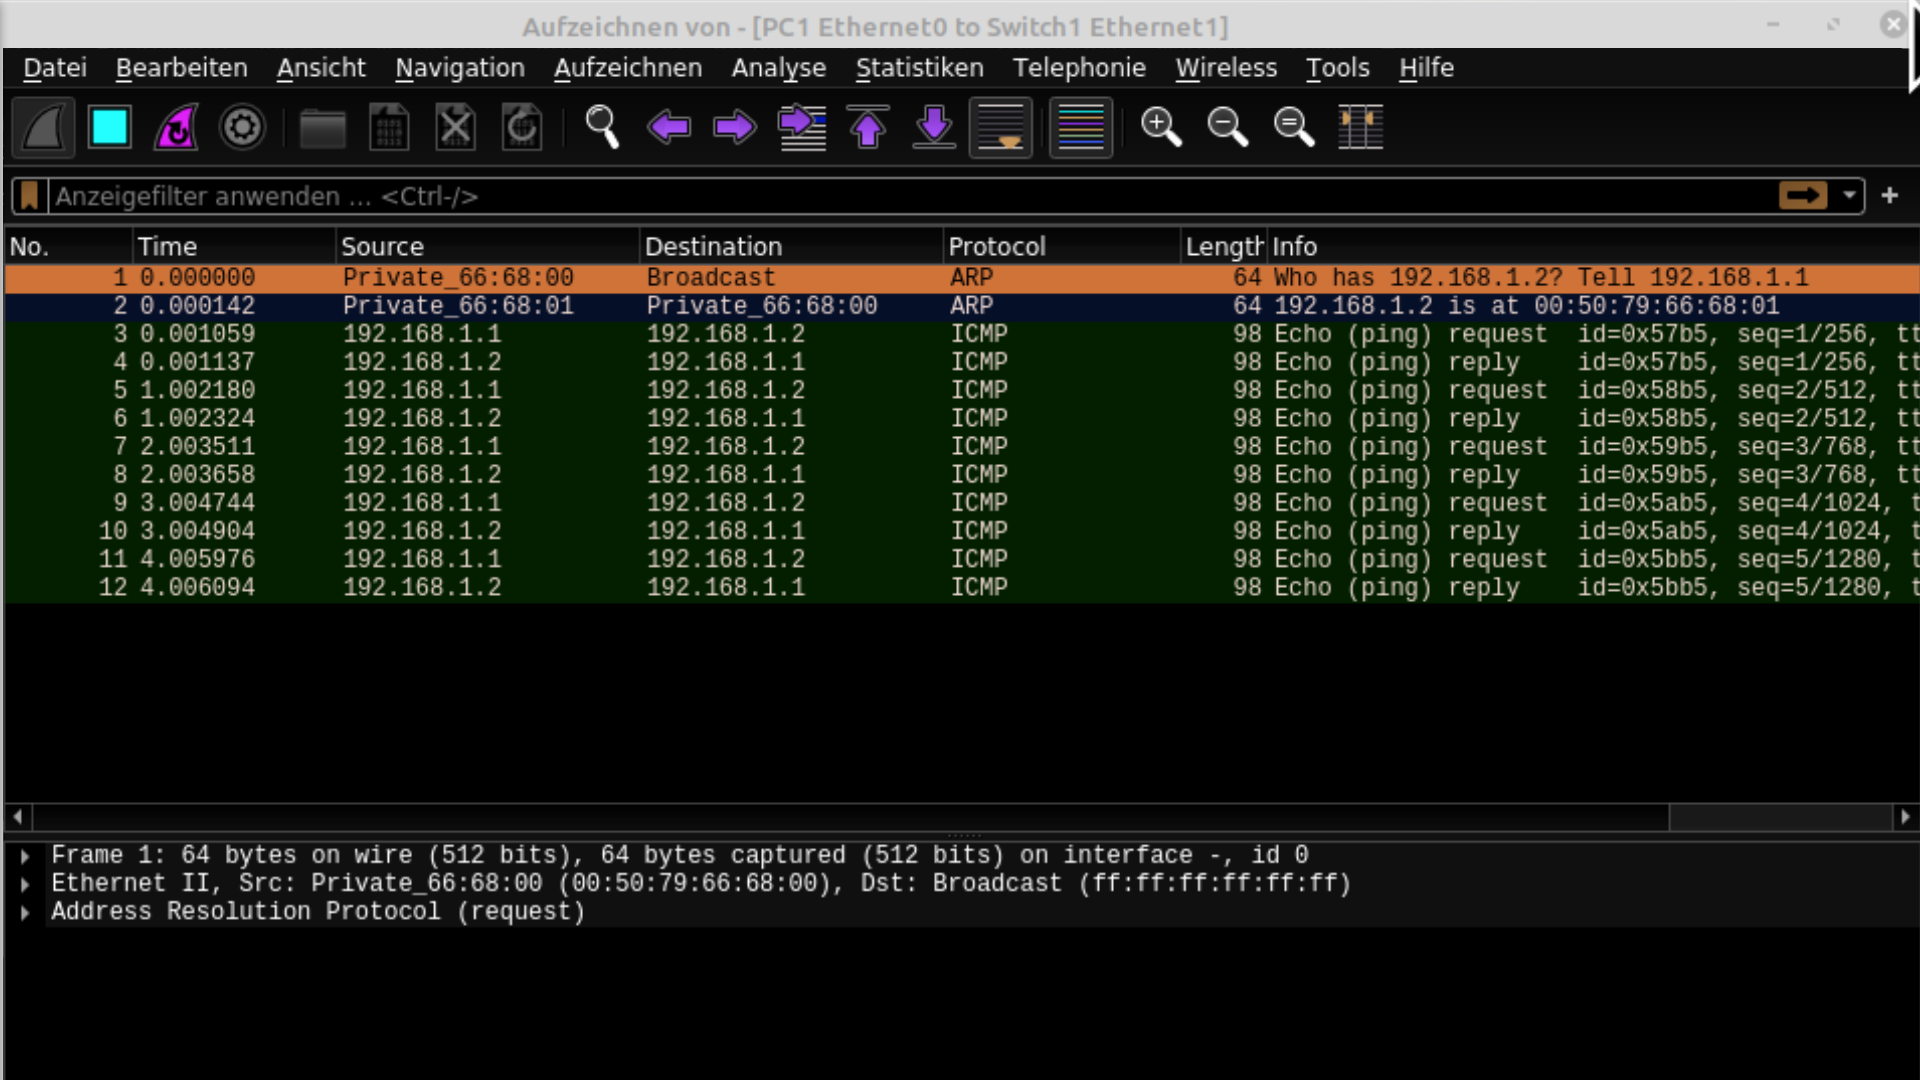
\includegraphics[width=\linewidth]{0501c01}
	\section*{Aufgabe 5.2}
	\subsection*{a)}
	Erweiterung des Netzwerks um einen weiteren PC. \\
	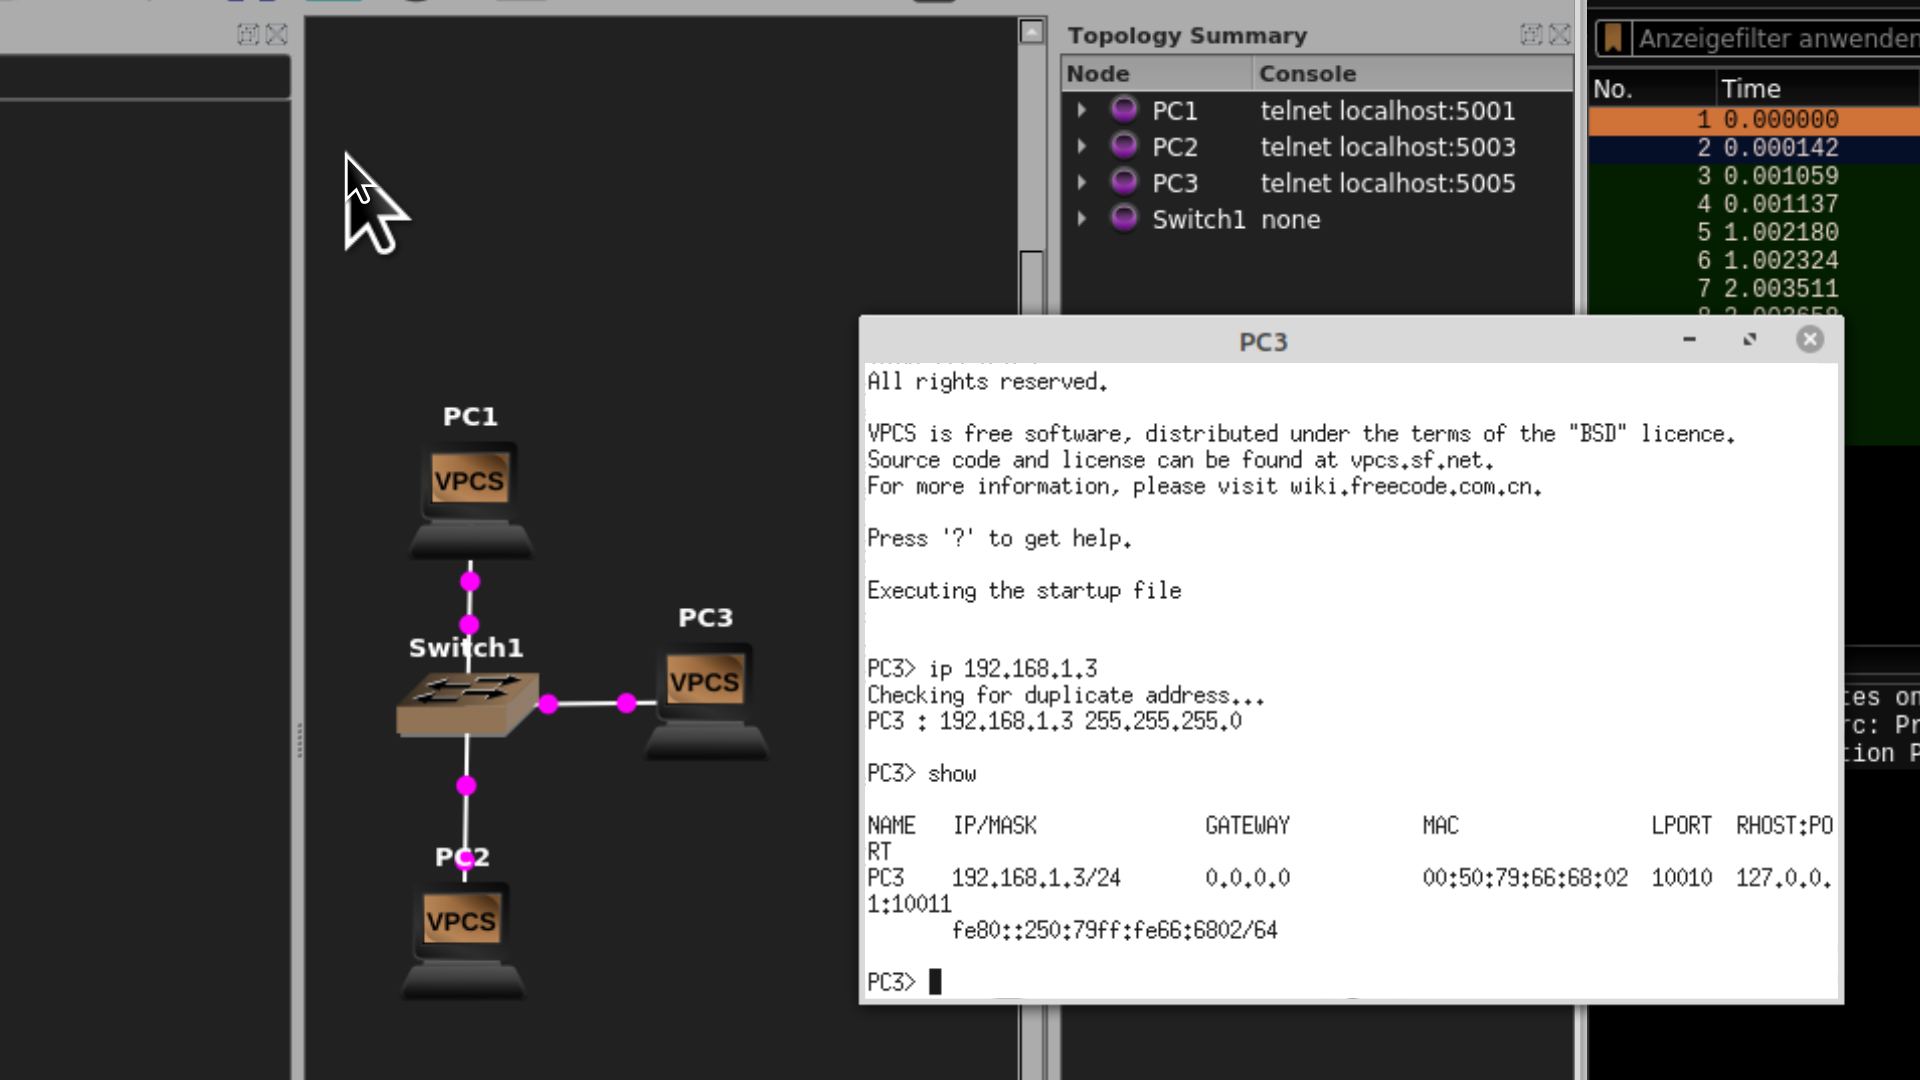
\includegraphics[width=\linewidth]{0502a01} \\
	Ping an den neuen PC3 von einem anderen PC aus. \\
	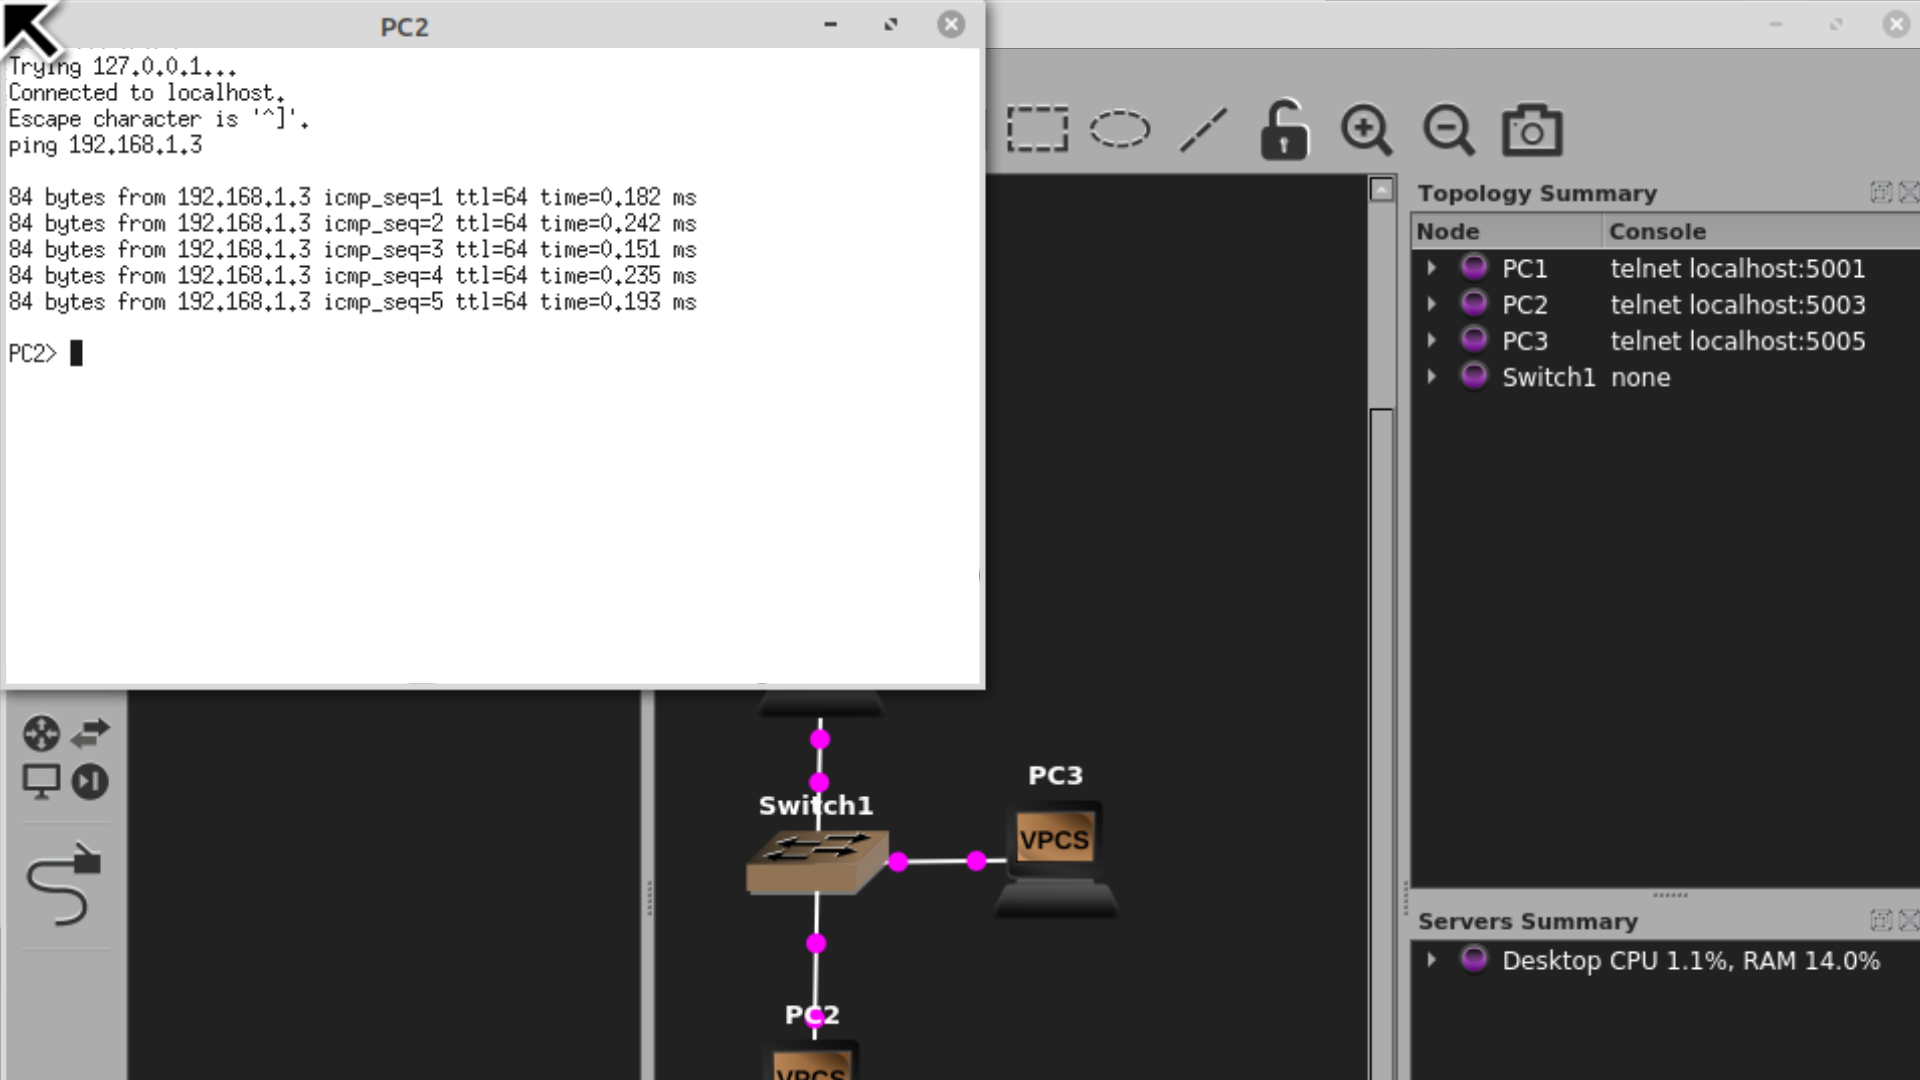
\includegraphics[width=\linewidth]{0502a02}
	\subsection*{b)}
	Pingversuch im V-Lan. Rechts mit PC3 an PC1 und links mit PC2 an PC1. \\
	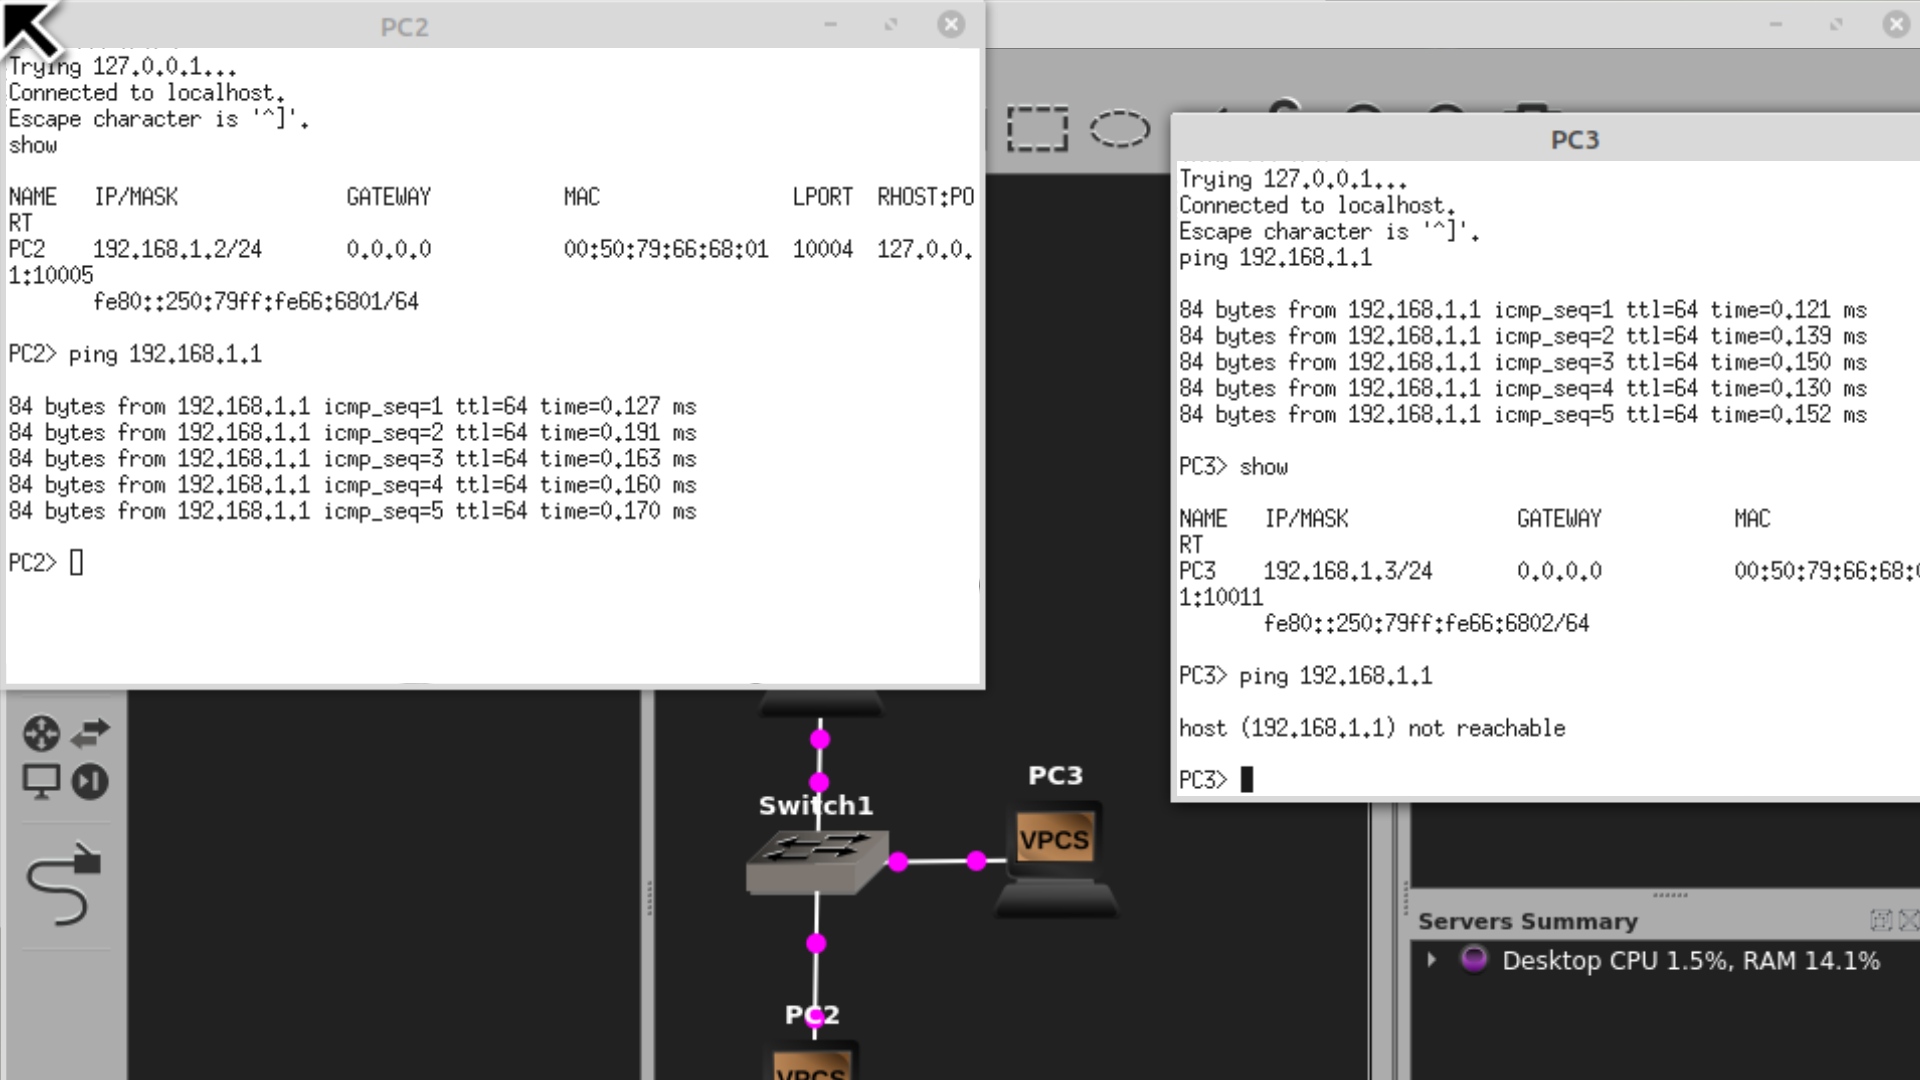
\includegraphics[width=\linewidth]{0502b01}
	\section*{Aufgabe 5.3}
	\subsection*{a)}
	Ping von PC4 auf PC1 über zwei Switches aufgezeichnet mit Wireshark. \\
	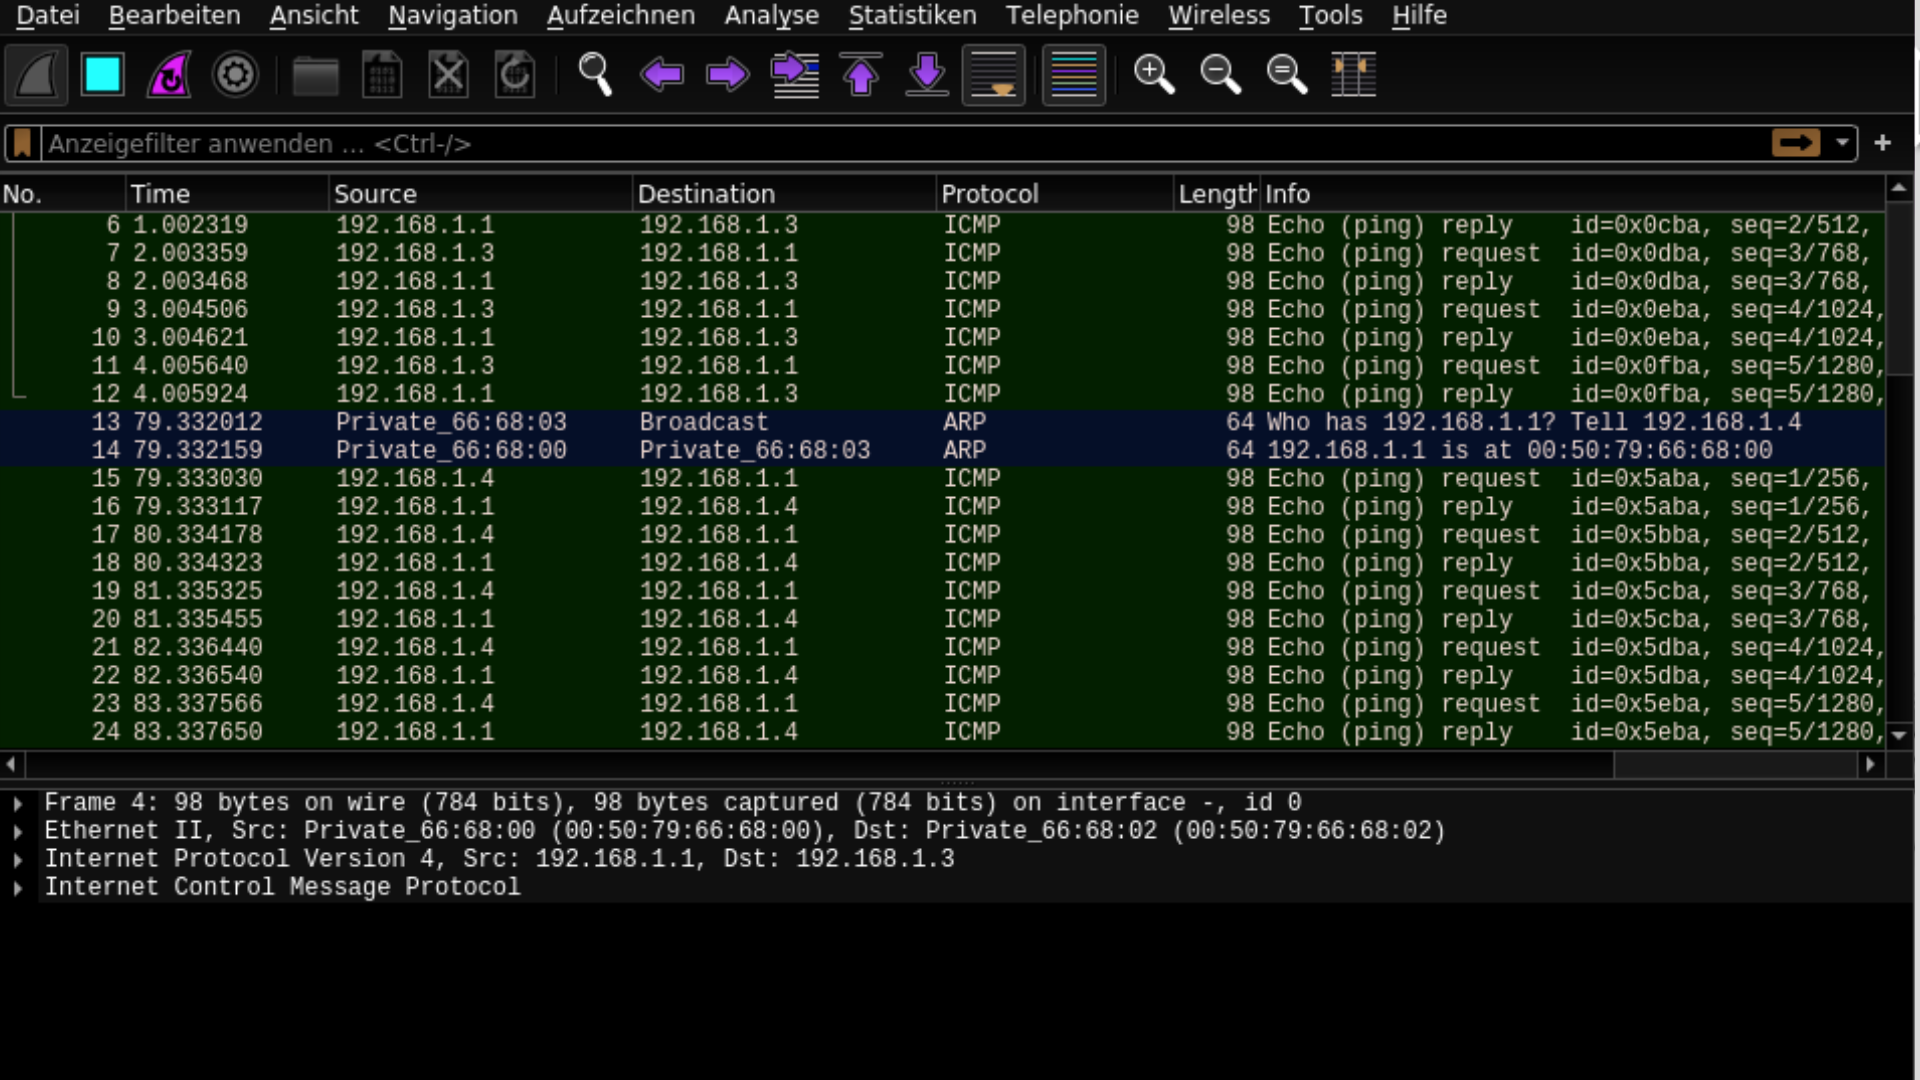
\includegraphics[width=\linewidth]{0503a01}
	\subsection*{b)}
	Ping innerhalb des V-Lans. Aufzeichnung mit Wireshark. Beispielhaft gezeigt: ping zwischen PC1 und PC4 \\
	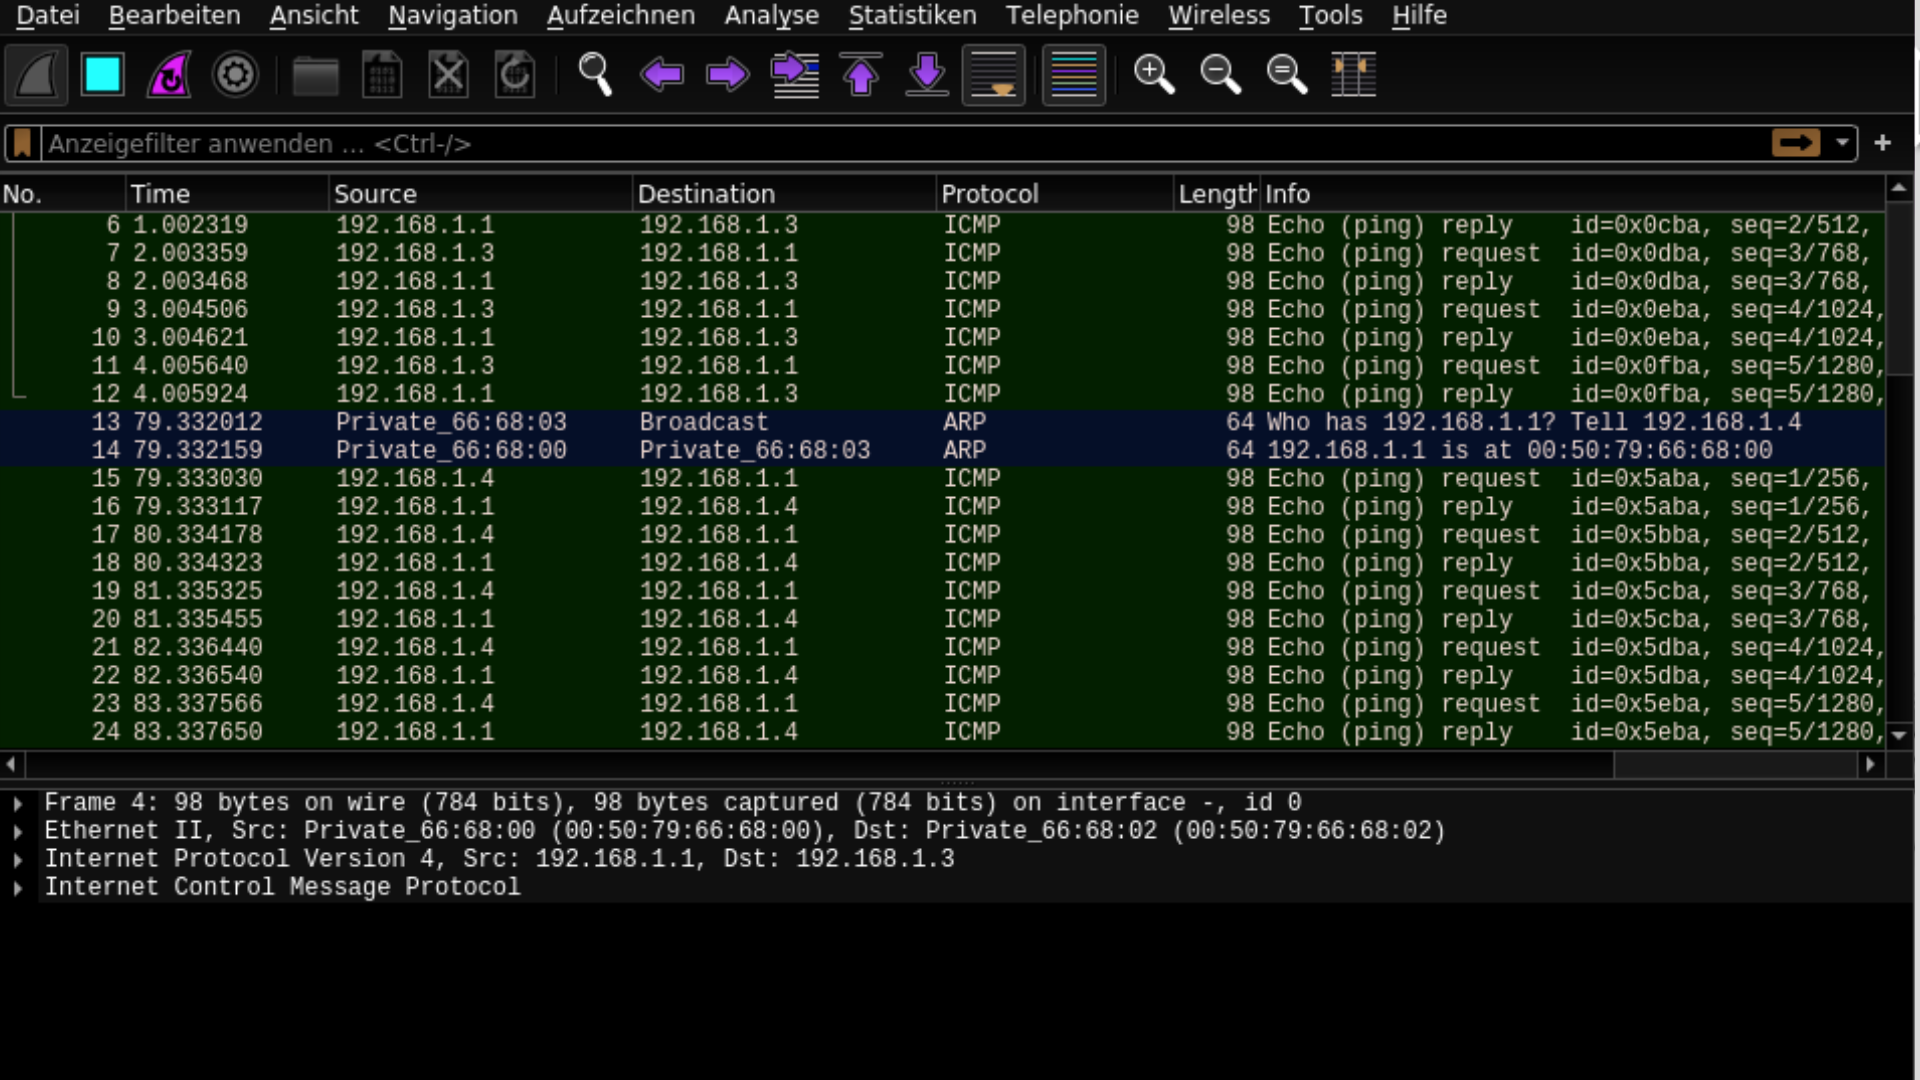
\includegraphics[width=\linewidth]{0503a01} \\
	Bei entsprechenden Paketen taucht im Hedder der Tag .1q auf.
\end{document}